\documentclass[10pt,twocolumn]{article}
\usepackage{fullpage,times,graphicx}

%opening

\begin{document}

\section*{High-Level GPGPU Programming with Parakeet}
We present Parakeet, an intelligent runtime library and JIT compiler which enables high-level languages such as Python's NumPy to take advantage of GPU acceleration while requiring no changes to existing code.

Parakeet is designed as an accelerator library for dynamic languages which possess either intrinsic array-oriented semantics or expressive array libraries. By array-oriented, we mean natively supporting both (1) array types; and (2) bulk array operators such as map, reduce, and scan for manipulating those arrays. Parakeet acts as an interpreter nested within its source language's execution context, allowing the programmer to continue using all of the source language's normal tools and support libraries.  At the moment, Parakeet has a front end for Q, an APL derivative widely used in financial computing.  Work is nearly completed on a front end for Python's NumPy.  We will present the NumPy front end at our session.

The program execution pipeline for Parakeet begins in the standard Python interpreter. The user simply imports the Parakeet library into the program.  At program start time, a subset of the program's function definitions are detected as parallelizable and are registered with Parakeet. The body of a registered function is then translated into an untyped intermediate representation using the Parakeet front end interface and Python's introspection facilities.

When a call is made to a function which has been registered with Parakeet, the untyped function is specialized by propagating type information from the arguments to all values in the body.  Type specialization translates the function into a typed intermediate language. Further standard optimizations are performed at this stage, the most impactful of which is \emph{array operator fusion}, wherein array operators are combined according to rewriting rules. This fusion step can be extremely beneficial to the final GPU program's performance, since it can potentially drastically improve the computational density of GPU programs and eliminate many wasteful array temporaries. 

Execution of the optimized typed IL is initiated by Parakeet's interpreter, which is then responsible for offloading certain operations onto the GPU. When the interpreter encounters an array operator it employs a cost-based heuristic (which considers nested array operators, data sizes, and memory transfer costs) to decide whether to execute that array operator on the GPU or CPU.

If an array operator's computation is deemed a good candidate for GPU execution, Parakeet flattens all nested array computations within that operator into sequential loops.  This payload is then inlined into a GPU program skeleton that implements that operator.  E.g., in the case of a \textbf{map} operation, Parakeet provides a skeletal algorithm that implements the pattern of applying the same function to each element of an array on the GPU.  The flattened payload function argument is inlined into this skeleton, and a complete GPU program is synthesized and JIT compiled.

To execute the GPU program, Parakeet first copies any of its inputs that aren't already present on the graphics card to the GPU's memory, which Parakeet treats as a managed cache of data present in the CPU's RAM. The GPU program is then executed, with its output lazily brought back to the CPU either when it is needed or when Parakeet's GPU garbage collector reclaims its space.

A further optimization performed by Parakeet is data layout manipulation.  GPU programs are extremely sensitive to memory access patterns, with orders of magnitude slowdowns if data is accessed inefficiently.  Parakeet is able to detect when an array's data layout (either row- or column-major) would lead to poor execution time and automatically transpose the array.  This optimization can lead to over an order of magnitude speedup in some cases.

We have evaulated Parakeet on various benchmark programs, and find that Parakeet delivers competitive performance even to hand-written CUDA code.  For example, the figure below details execution times for a K-Means algorithm hand-written in CUDA and as executed by Parakeet.  For this benchmark, Parakeet's performance is even better than the hand-written code as Parakeet makes better dynamic decisions as to where each portion of the algorithm (CPU or GPU) would best be run.

\begin{figure}[h!]
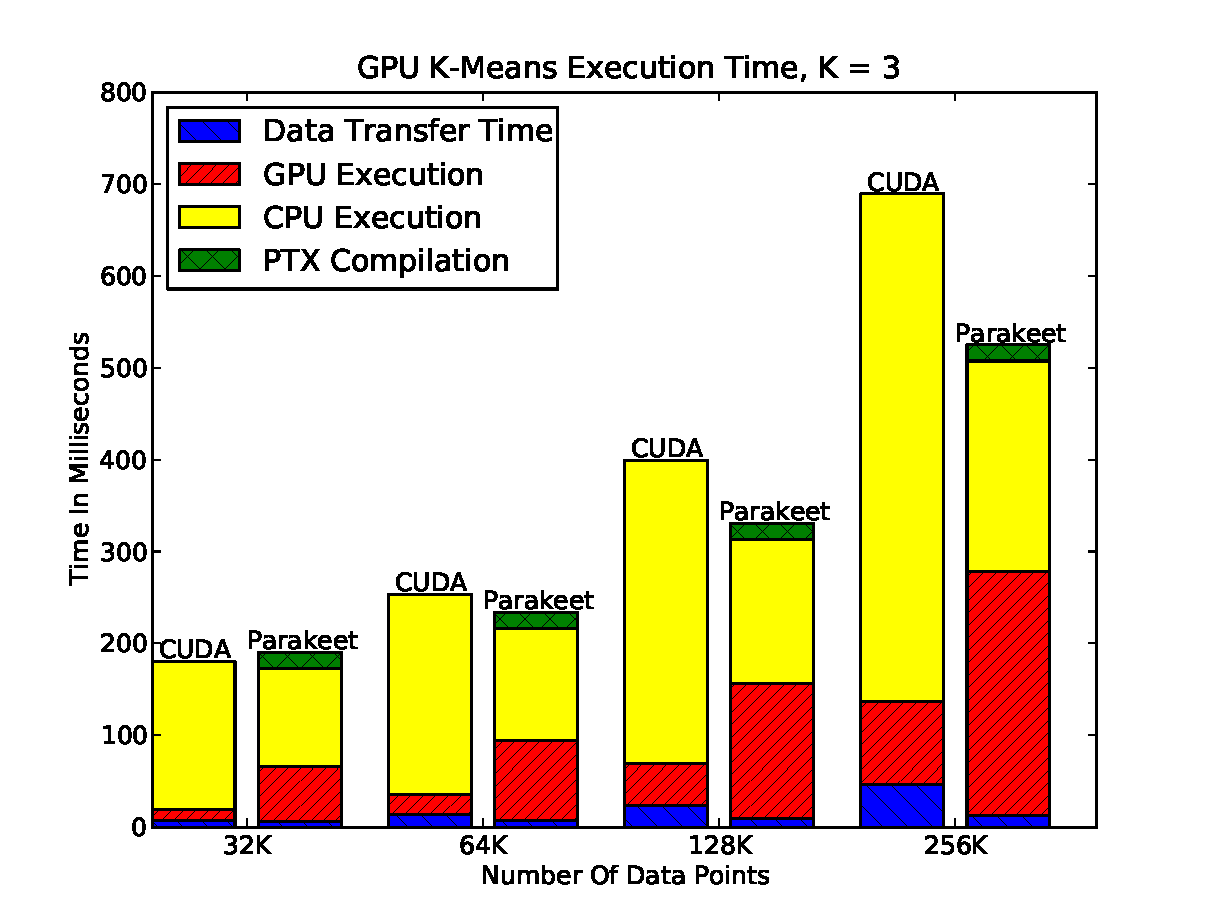
\includegraphics[scale=0.4]{KMGPU.pdf}
\label{BSGPU}
\end{figure}

At our session next year, we plan on detailing our in-progress support for handling computations whose data requirements are larger than those of GPU memory as well as the use of multiple GPUs.

\end{document}
